\chapter{Implementierung}\label{ch:implementierung}
Das folgende Kapitel beschreibt die eigene Entwicklung einer Indexstruktur zur Optimierung der \textit{k}-Nächsten-Nachbarn-Suche nach Bloom-Filtern in AMBIENCE. Sie heißt \textit{BloomFilterTree}. Abschnitt \ref{sec:aufbau} beschreibt den konzeptionellen Aufbau. Die praktische Umsetzung wird in Abschnitt\ref{sec:umsetzung} dargestellt. Die zentralen Operationen zum Einfügen von Bloom-Filtern und die \textit{k}-nächste-Nachbarn-Suche werden in den Abschnitten \ref{sec:einfügen} und \ref{sec:knn} erläutert. Abschließend wird dargestellt, welche alternativen Ansätze während der Implementierung verfolgt und weshalb sie letztlich verworfen wurden (vgl. Abschnitt \ref{sec:alternativen}). Evaluation des Verfahrens und Gegenüberstellung mit der naiven Implementierung finden sich im folgenden Kapitel \ref{ch:evaluation}.  
\section{BloomFilterTree}\label{sec:bloom-filter-tree}
Um möglichst plattformunabhängig zu bleiben, wurde die Implementierung in C++ realisiert. Ausgewählte Codebeispiele finden sich im Anhang (vgl. Kapitel \ref{ch:anhang}). Zunächst war überlegt worden, teilweise auf bestehende Bibliotheken für Bloom-Filter und Baumstrukturen zurückzugreifen wie die bekannte \textit{Open Bloom Filter}-Bibliothek von Arash Partow\footnote{Vgl. \url{https://github.com/ArashPartow/bloom} für den Quellcode.}. Darauf wurde schließlich aus zwei Gründen verzichtet: Erstens liegt der Fokus der Arbeit nicht auf der Implementierung von Bloom-Filtern, sondern sie dienten als Schnittstelle. Durch die Verwendung bestehender Bibliotheken wäre außerdem zu befürchten, dass Messergebnisse einerseits durch den Rechnenaufwand für nicht benötigte Operationen, andererseits durch in AMBIENCE nicht vorhandene Optimierungen verfälscht würden. 

Eine Bibliothek für B$^+$-Bäume ist z.B. das \textit{STX B+ Tree package} von Timo Bingmann\footnote{Vgl. \url{https://github.com/bingmann/stx-btree} für den Quellcode.}. Wie in Abschnitt \ref{sec:bloom-index} 
dargestellt, existieren keine bekannten Varianten von Indexstrukturen, die sich unverändert für AMBIENCE übernehmen ließen. Auch eine bestehende Bibliothek müsste also stark abgewandelt werden. Gleichzeitig könnten dieselben Verfälschungen auftreten wie bei Verwendung einer Bloom-Filter-Bibliothek. So wurde auch davon abgesehen.
\subsection{Aufbau}\label{sec:aufbau} 
Am vielversprechendsten erschien es, wie Sakuma und Sato in ihrer Arbeit über "`Structured Bloom Filters Based on Similarity"'\footnote{Vgl. \cite{Sakuma2011}.} zunächst von einem B$^+$-Baum auszugehen (vgl. Abschnitt\ref{sec:bloom-index}). Dieser wurde zuerst implementiert mit allen Eigenschaften wie in Abschnitt \ref{sec:indexstrukturen} beschrieben. Anschließend wurde er schrittweise für die Organisation der Bloom-Filter erweitert: 
\begin{enumerate}
	\item Die Datensätze sind Bloom-Filter, d.h. die jedes Blatt enhält Zeiger auf die \textit{n} Bloom-Filter-Objekte, die darin eingefügt wurden. Bloom-Filter-Objekte werden über ihre ID als Primärschlüssel identifiziert. 
	\item Jeder Baumknoten hat einen Vereinigungs-Bloom-Filter. Er wird aus dem bitweisen logischen Oder aller Bloom-Filter gebildet, die in den darunter liegenden Teilbaum eingefügt wurden (vgl. Abschnitt \ref{sec:bloom-index}).
\end{enumerate}
Abb. \ref{fig:pic6} veranschaulicht den Aufbau eines BloomFilterTree. Die Baumknoten sind darin blau markiert. Sie enhalten die Primärschlüssel der Bloom-Filter sowie Zeiger auf die Kind- bzw. Nachbarknoten. Jeder Knoten hat einen weiß markierten Vereinigungs-Bloom-Filter. Die tatsächlichen Datensätze sind violett markierte Bloom-Filter. Die Blätter verweisen jeweils auf die darin eingefügten Filter.
\begin{figure}[hpbt]
  \centering
  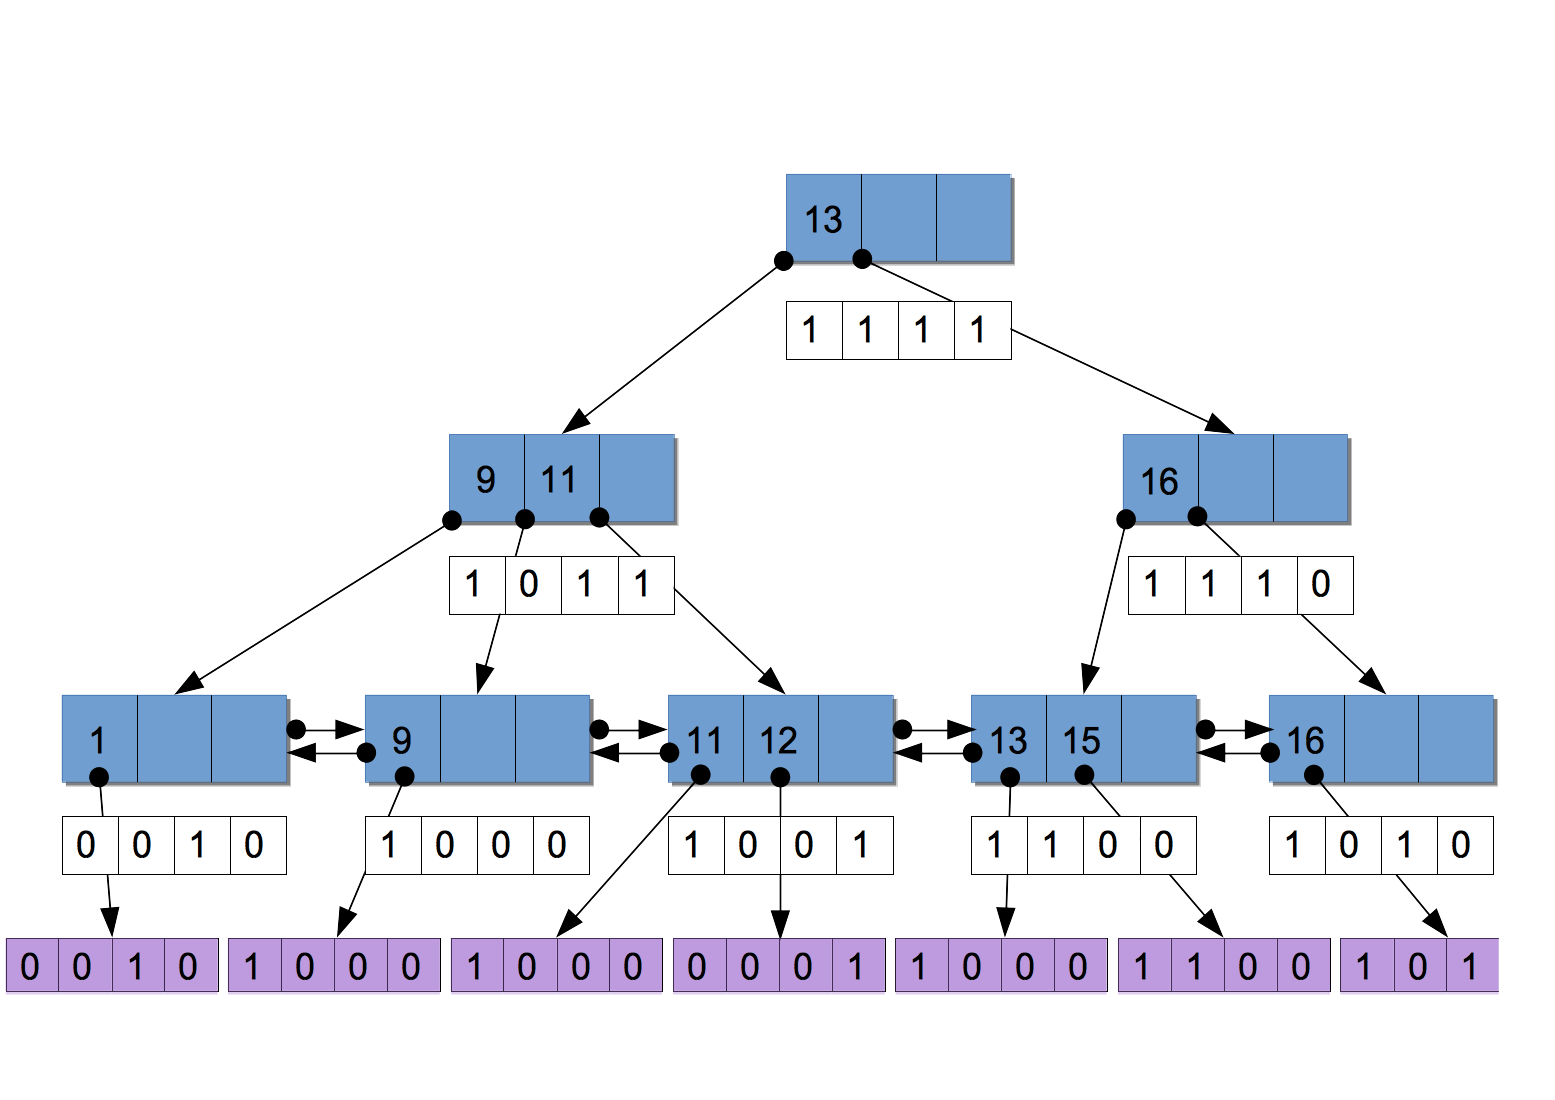
\includegraphics[width=1.0\textwidth]{pictures/bloom-filter-tree2.png}\\
  \caption[Aufbau eines BloomFilterTree]{Aufbau eines BloomFilterTree mit Bloom-Filtern als Datensätzen und Vereinigungs-Bloom-Filtern an allen Knoten.}\label{fig:pic6}
\end{figure}
\subsection{Umsetzung}\label{sec:umsetzung}
Die Klasse \texttt{BloomFilterTree} enthält schließlich alle notwendigen Parameter und Operationen zur Organisation der Bloom-Filter. Dazu gehören die B$^+$-Baum-Operationen wie Einfügen und Suchen von Schlüsseln, Traversieren der Blätter, boolesche Abfrage nach Enthaltensein eines Schlüssel im Baum, Zählen der Blätter und viele mehr. Darüber hinaus gibt es zahlreiche weitere Methoden: 
\begin{enumerate}
	\item \textit{Management-Methoden} zum Berechnen der Jaccard-Distanzen zu allen Filtern im Baum, k-Nächste-Nachbarn-Suche in der naiven Version, Traversieren der Datensätze (also der Bloom-Filter) etc..
	\item Die \textit{zentralen Methoden} des Verfahrens: Einfügen der Bloom-Filter nach Ähnlichkeit und \textit{k}-Nächste-Nachbarn-Suche. 
	\item \textit{Mess- und Vergleichsmethoden}, z.B. um die Varianten der \textit{k}-Nächste-Nachbarn-Suche, die Aufbaukosten und den Speicherbedarf der Datenstrukturen zu vergleichen. 
\end{enumerate}
Die Header-Datei der Klasse \texttt{BloomFilterTree} ist im Anhang abgedruckt (vgl. Abschnitt \ref{sec:BloomFilterTree.hpp}). In der Klasse \texttt{BloomFilter} wurden alle Parameter und Operationen auf Bloom-Filtern realisiert, die sich im Laufe der Arbeit als wichtig erwiesen. Dazu gehören: 
\begin{enumerate}
	\item \textit{Typische Bloom-Filter-Parameter und -Methoden} wie Anzahl der Hashfunktionen, Daten-Array und Setzen von Bits.
	\item \textit{Mathematische Methoden und Vergleichsoperationen} wie Berechnung von Teil- und Obermengen, bitweises logisches Und und Oder, Berechnung und Abschätzung der Jaccard-Distanz etc..
	\item \textit{Methoden zum Bloom-Filter-Management} wie Einfügen von zufälligen Elementen aus einem Wörterbuch, zufällige Initialisisierung mit Werten aus $\{0,1\}$ usw..
\end{enumerate}
Die Header-Datei der Klasse \texttt{BloomFilter} ist im Anhang abgedruckt (vgl. Abschnitt \ref{sec:BloomFilter.hpp}).
\subsection{Einfügen}\label{sec:einfügen}
Das Verfahren zum Einfügen zählt zu den wichtigsten Methoden der Indexstruktur und ist entscheidend für die Optimierung von Laufzeit und CPU-Zeit der \textit{k}-Nächste-Nachbarn-Suche. Der Algorithmus basiert auf den Teil- und Obermengenbeziehungen zwischen Bloom-Filtern und nutzt die Vereinigungs-Bloom-Filter der bereits existierenden Knoten, um die optimale Position zum Einfügen eines neuen Bloom-Filters in den BloomFilterTree zu finden: Falls der Baum noch leer ist, wird ein neuer Blattknoten erstellt und das Bloom-Filter-Objekt als erstes Datenobjekt dort eingefügt. Der neue Knoten wird die Wurzel des BloomFilterTree. Andernfalls wird ausgehend vom Wurzelknoten rekursiv die optimale Position für den Bloom-Filter im Baum gesucht. Dazu werden die Teil- und Obermengen-IDs des Filters berechnet. Dem Filter wird die neue Teilmengen-ID zugewiesen er wird gemäß der B$^+$-Baum-Regeln in den Baum eingefügt. Sind Teilmengen- und Obermengen-IDs unterschiedlich, wird ein zweites Datenobjekt mit der Obermengen-ID erstellt und ebenfalls in den Baum eingefügt. Falls der BloomFilterTree während des Einfügens um eine Ebene gewachsen ist, wird der Elternknoten des alten Wurzelknoten zur neuen Wurzel. Abbildung \ref{fig:pic7} verdeutlicht den Ablauf des Einfüge-Algorithmus:  
%\begin{figure}[hpbt]
%  \centering
%  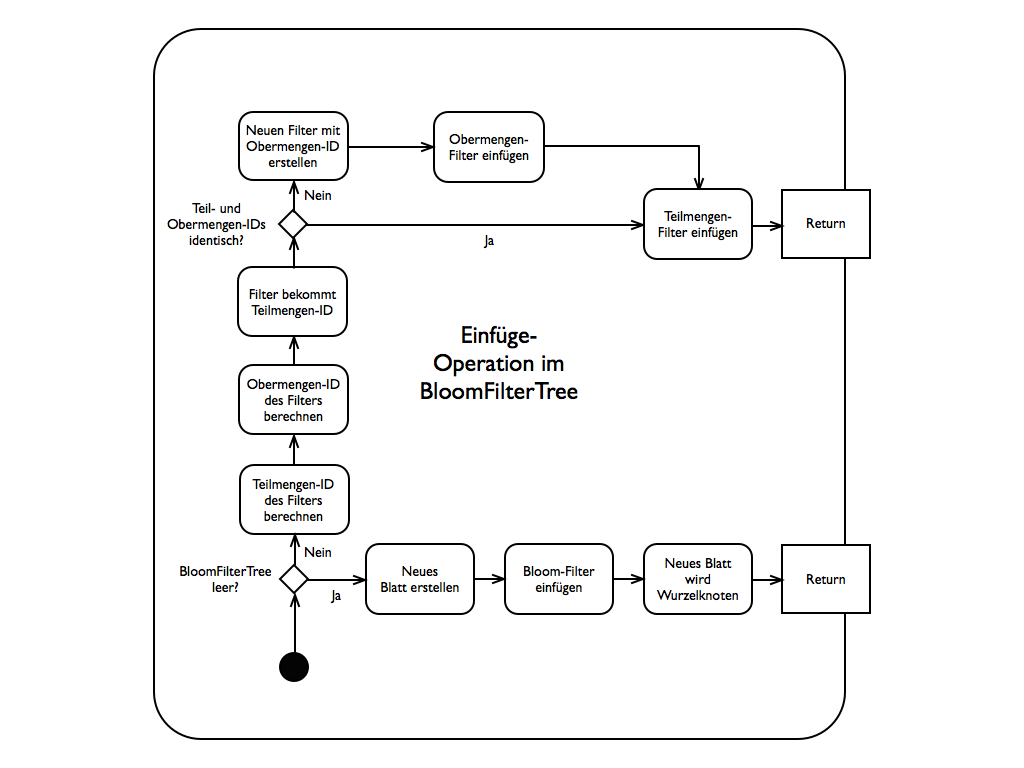
\includegraphics[width=0.9\textwidth]{pictures/insert-as-sets.png}\\
%  \caption[Einfügen von Objekten im BloomFilterTree]{Einfügen von Objekten im BloomFilterTree.}\label{fig:pic7}
%\end{figure}
Die Hauptarbeit des Einfügens findet in den Blattknoten statt, wo die optimalen Teilmengen- und Obermengen-IDs der Filter berechnet werden. Die Funktion \texttt{computeSubsetId()} der Klasse \texttt{BloomFilterLeaf} ist beispielhaft im Anhang abgedruckt (vgl. \ref{sec:computeSubsetId()}). Sie dient der Berechnung der optimalen Teilmengen-ID eines einzufügenden Bloom-Filters. Die Funktion \texttt{computeSupersetId()} berechnet in ähnlicher Weise die optimale Obermengen-ID. Dabei werden folgende Schritte ausgeführt: 
\subsection{k-Nächste-Nachbarn-Suche}\label{sec:knn}
%\begin{figure}[hpbt]
%  \centering
%  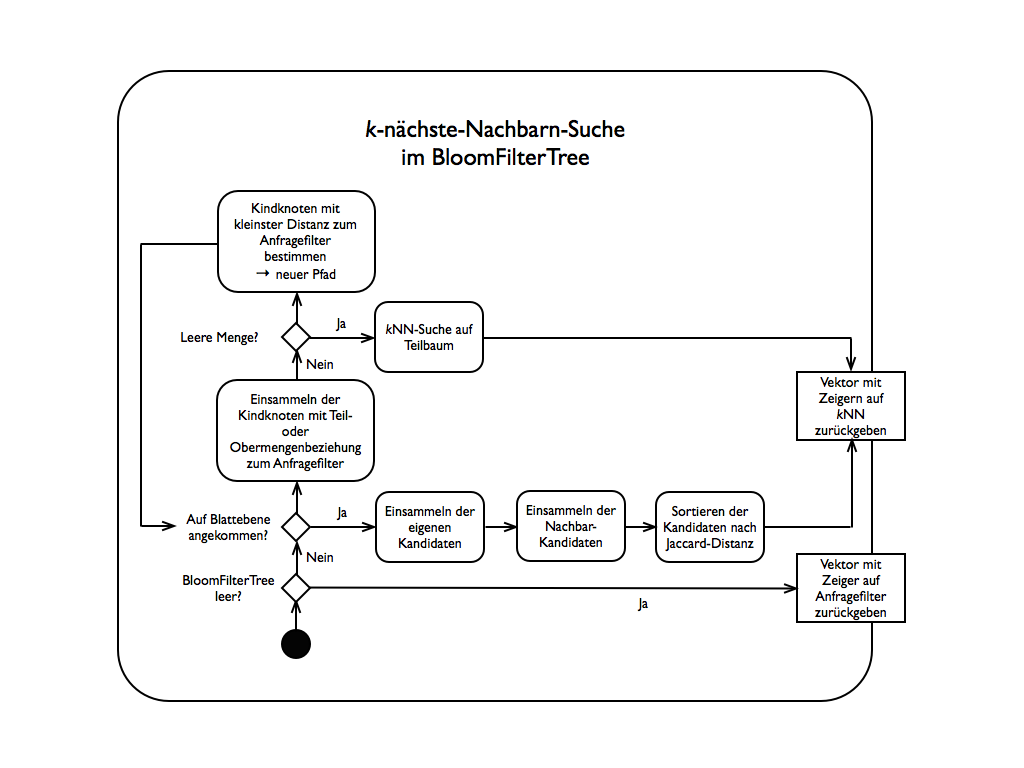
\includegraphics[width=0.9\textwidth]{pictures/knn.png}\\
%  \caption[\textit{k}-Nächste-Nachbarn-Suche im BloomFilterTree]{\textit{k}-Nächste-Nachbarn-Suche im BloomFilterTree.}\label{fig:pic8}
%\end{figure}
\section{Alternative Ansätze}\label{sec:alternativen}
\subsection{Einfügen gemäß Jaccard-Distanzen}\label{sec:ähnlichkeit}
\subsection{Doppelt verkettete Liste}\label{sec:verkettete-liste}
%%Es lassen sich auch mehrere Bilder nebeneinander platzieren wie z.B. in Abbildung
%%\ref{fig:multipic} zu sehen ist.
%%\begin{figure}[hpbt]
%% \centering
%%  %%----start of first subfigure----
%%  \subfloat[FIFO size limited to 20 entries]{
%%   \label{fig:multipic:a} %% label for first subfigure
%%   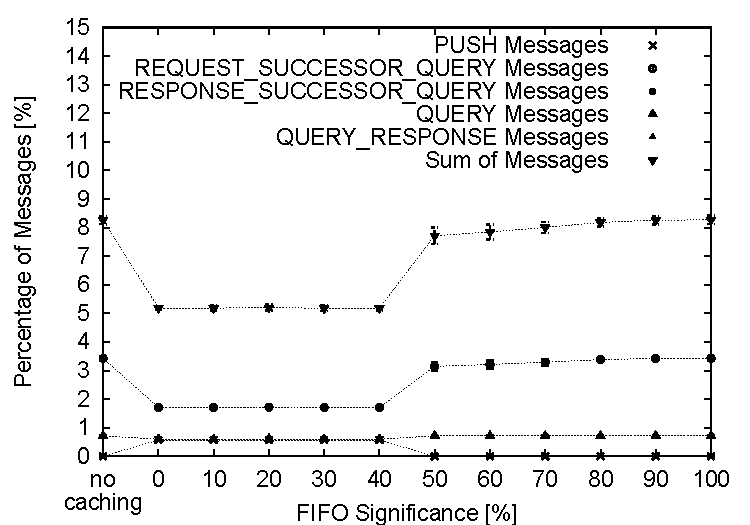
\includegraphics[width=0.48\linewidth]{pic1}}
%%  \hspace{0.01\textwidth}
%%  %%----start of second subfigure----
%%  \subfloat[FIFO size limited to 30 entries]{
%%   \label{fig:multipic:b} %% label for second subfigure
%%   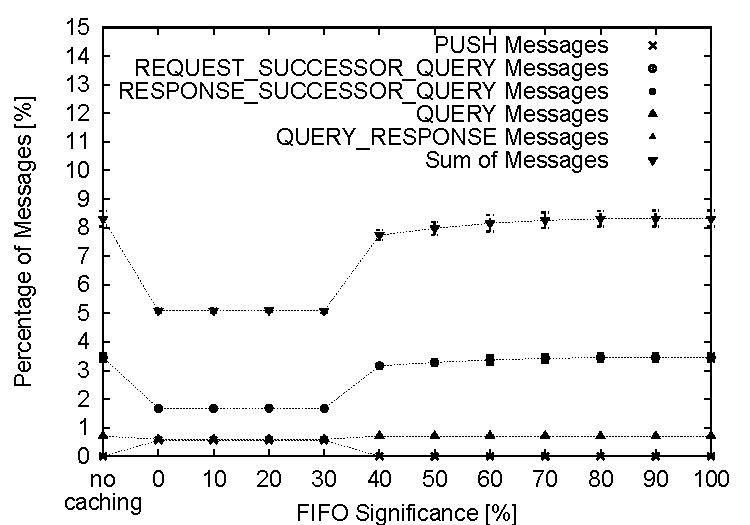
\includegraphics[width=0.48\linewidth]{pic2}}\\[0pt] % horizontal break
%%  %%----start of third subfigure----
%%  \subfloat[FIFO size limited to 40 entries]{
%%   \label{fig:multipic:c} %% label for third subfigure
%%   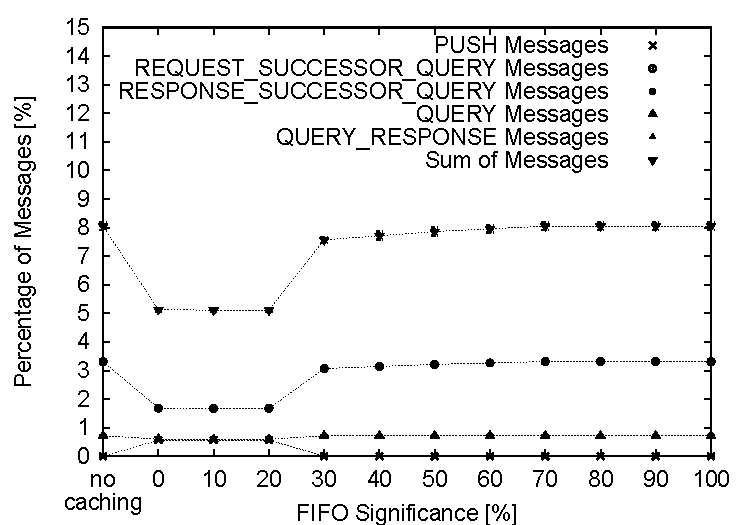
\includegraphics[width=0.48\linewidth]{pic3}}
%%  \hspace{0.01\textwidth}
%%  %%----start of fourth subfigure----
%%  \subfloat[FIFO size limited to 50 entries]{
%%   \label{fig:multipic:d} %% label for fourth subfigure
%%   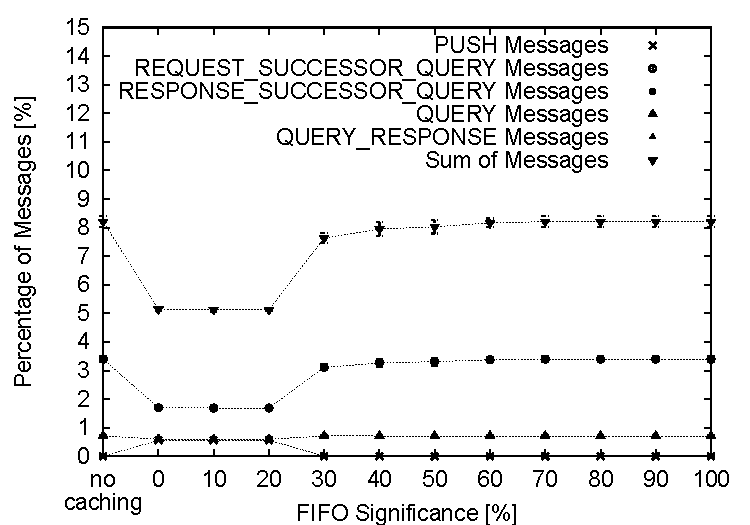
\includegraphics[width=0.48\linewidth]{pic4}}
%% \caption[Observed message fractions and 95\% confidence intervals for Chord]{Observed message fractions and 95\% confidence intervals for Chord without the influence of churn. The FIFO capacity varies from 20 (\ref{fig:multipic:a}) -- 50 (\ref{fig:multipic:d}) entries (decadic steps).}
%% \label{fig:multipic} %% label for entire figure
%%\end{figure}
%%
%%\subsection{Programm Code}
%%Eine elegante Möglichkeit, Programmtext einzubinden, lässt sich mit dem listings-Paket erreichen.
%%Das \verb|HelloWorld| Programm aus Listing \ref{lst:hw} hat in Zeile \ref{line:hw3} übrigens einen Programmierfehler.
%%\begin{lstlisting}[float=htp,caption=Hello World,label=lst:hw,language=Java, numbers=left, numberstyle=\tiny, stepnumber=2, numbersep=8pt, escapeinside={//@}{@//},backgroundcolor=\color{yellow},xleftmargin=3ex,xrightmargin=1ex]
%%public class HelloWorld {
%%    public static void main(String[] args) {
%%        Syste.out.println("Hello, World"); //@\label{line:hw3}@//
%%    }
%%}
%%\end{lstlisting}
%
